\chapter{A wavepacket based algorithm}
\label{ch:wave_packet_based_algorithms}

With the detailed insight from the last chapter we now move on and see how we can
use semiclassical wavepackets to solve the vector valued Schrödinger equation
as defined by \eqref{eq:basics_tdse_vector}. In this chapter we will study an
algorithm that was presented in reference \cite{FGL_semiclassical_dynamics}. It uses the
semiclassical wavepackets from the last chapter to simulate the time evolution
of an initial wavepacket.

\section{Splitting the Schrödinger equation}

The linear time dependent Schrödinger equation as defined by \eqref{eq:basics_tdse_semi}
with a splitting of the Hamiltonian operator $H$ into a kinetic and a potential part
as in equation \eqref{eq:basics_def_ops} can be written as two separate equations.

The first equation that contains only the kinetic operator $T$ describes the time
evolution of a free particle:

\begin{equation} \label{eq:tdse_free_particle}
  i \varepsilon^2 \frac{\partial \Psi}{\partial t} = - \frac{1}{2} \varepsilon^4 \frac{\partial^2}{\partial x^2} \Psi \,.
\end{equation}

The other part contains only the potential $V\ofs{x}$ and reads:

\begin{equation} \label{eq:tdse_potential_part}
  i \varepsilon^2 \frac{\partial \Psi}{\partial t} = V\ofs{x} \Psi \,.
\end{equation}

\subsection{Splitting of the potential}

The next step is to additionally decompose the potential. We split $V$ into a
local quadratic Taylor approximation $U\ofs{x}$ and the non-quadratic remainder
$W\ofs{x}$ as:

\begin{equation}
  V\ofs{x} = U\ofs{x} + W\ofs{x} \,.
\end{equation}

This yields two new potential equations that replace \eqref{eq:tdse_potential_part},
one with the quadratic part of the potential which, of course, describes an
harmonic oscillator:

\begin{equation} \label{eq:tdse_quadratic}
  i \varepsilon^2 \frac{\partial \Psi}{\partial t} = U\ofs{x} \Psi \,.
\end{equation}

The other equation contains all the bulky pieces that remain after the splitting:

\begin{equation} \label{eq:tdse_remainder}
  i \varepsilon^2 \frac{\partial \Psi}{\partial t} = W\ofs{x} \Psi \,.
\end{equation}

\section{Propositions about exact propagation}

The benefit of this two levels of decomposition becomes obvious once we recall that
the aim is to propagate semiclassical wavepackets. It turns out that two out of
these three parts can be solved exactly. In this section we closely follow reference
\cite{FGL_semiclassical_dynamics}.

We can solve the free particle equation \eqref{eq:tdse_free_particle} exactly.
The important point is that if the wave function has the form of a semiclassical
wavepacket defined by equation \eqref{eq:hagedorn_kstate_1d} then the coefficients
$c_i$ won't change during time propagation. For the time evolution during a single
time step $\tau$ we get the following equations

\begin{equation} \label{eq:splitting_prop_kinetic}
\begin{split}
  q\ofs{t+\tau} & = q\ofs{t} + \tau p\ofs{t} \\
  Q\ofs{t+\tau} & = Q\ofs{t} + \tau P\ofs{t} \\
  S\ofs{t+\tau} & = S\ofs{t} + \frac{1}{2} \tau p\ofs{t}\T p\ofs{t}
\end{split}
\end{equation}

with $p$ and $P$ being constant.

In a similar way we can solve the quadratic potential equation \eqref{eq:tdse_quadratic}
exactly without changing the packet's coefficients $c_i$. The time evolution this
time reads

\begin{equation} \label{eq:splitting_prop_harmonic}
\begin{split}
  p\ofs{t+\tau} & = p\ofs{t} - \tau \nabla U\ofs{q\ofs{t}} \\
  P\ofs{t+\tau} & = P\ofs{t} - \tau \nabla^2 U\ofs{q\ofs{t}} Q \ofs{t} \\
  S\ofs{t+\tau} & = S\ofs{t} - \tau U\ofs{q\ofs{t}}
\end{split}
\end{equation}

where $q$ and $Q$ stay the same.

During these two parts we only change the parameters $P$, $Q$ and the phase $S$
besides the position $q$ and momentum $p$ of the wavepacket but we never touch
the coefficients $c_i$.

In the third step which deals with equation \eqref{eq:tdse_remainder} however, we
can no longer keep the coefficients $c_i$ constant. But in this turn, we can fix
the five parameters and solely update the coefficients. The starting point is
the following variational approximation

\begin{equation} \label{eq:variational_approximation}
  \dotp{\phi_k}{i\varepsilon^2 \frac{\partial u}{\partial t} - W u} = 0 \quad \forall k
\end{equation}

on the Hilbert space $\mathcal{M}$ defined by

\begin{equation} \label{eq:hagedorn_space}
  \mathcal{M} \assign \{v \in L^2\ofs{R^d} : v\ofs{x} = \sum_{k=0}^{K-1} c_k \phi_k\ofs{x} \} \,.
\end{equation}

This is the space spanned by all functions defined by \eqref{eq:hagedorn_kstate_1d}
with identical and fixed parameters $P$, $Q$, $p$ and $q$. Equivalently to \eqref{eq:variational_approximation}
we can solve the following system of linear ordinary differential equations

\begin{equation} \label{eq:ode_for_coeffs}
  i \varepsilon^2 \frac{d c_k}{dt} = \sum_{l=0}^{K-1} f_{k,l} c_{l}
\end{equation}

where $f_{k,l} \assign \Braket{\phi_k | W | \phi_l}$ and we collect all these $f$
into a Hermitian matrix $F$ which is the matrix representation of the non-quadratic
remainder $W$ over the basis $\{\phi_i\}_i$. The solution to \eqref{eq:ode_for_coeffs} is then simply given by

\begin{equation} \label{eq:splitting_prop_remainder}
  c\ofs{t+\tau} = \exp\ofs{-\frac{i\tau}{\varepsilon^2}F} c\ofs{t}
\end{equation}

and describes the time evolution of the coefficients in the potential's remainder.

For the exact details and the proofs about this splitting and the separate
time evolutions we refer to section 2 of \cite{FGL_semiclassical_dynamics}.

\subsection{The matrix representation}

One last step remains before we can put together the algorithm. In the last paragraph
above we need the matrix denoted by $F$. The definition gives us this equation:

\begin{equation} \label{eq:the_matrix_f}
  f_{k,l} \assign \Braket{\phi_k | W | \phi_l} = \int_{\mathbb{R}^d} \conj{\phi_k\ofs{x}} W\ofs{x} \phi_l\ofs{x} dx
\end{equation}

which looks like any integration problem. We now want to find an efficient way to calculate this
integral for all $k$ and $l$ or, in other words, set up the matrix $F$. The integral containing
$W$ can almost never be solved analytically thus the integral is approximated by quadrature. Because
we will need the results at different places, let's look at a much broader setup of this problem.

\section{Analytical integration and quadrature}

Suppose we have the wave function $\Ket{\Phi_i}$ of a component as defined by \eqref{eq:hawp_def_single}.
Recall then for the basis functions we have orthogonality: $\Braket{\phi_m | \phi_n } = \delta_{m,n}$. The
two kets $\Ket{\Phi_i}$ and $\Ket{\Phi_j}$ must have the same Hagedorn parameters
for the time being, but of course they can have different coefficients. Thus we add
upper indices to the coefficients. For a general but sufficiently smooth function

\begin{align*}
  f : \mathbb{R} & \rightarrow \mathbb{R} \\
               x & \mapsto f \ofs{x}
\end{align*}

we want to transform the following expression into an integral

\begin{equation} \label{eq:inner_product_single_family}
\begin{split}
  \Braket{ \Phi_i | f | \Phi_j } & = \Braket{e^\frac{iS}{\varepsilon^2} \sum_k c_k^i \phi_k | f | e^\frac{iS}{\varepsilon^2} \sum_k c_k^j \phi_k} \nonumber \\
                                 & = \underbrace{e^\frac{-iS}{\varepsilon^2} e^\frac{iS}{\varepsilon^2}}_{=1} \Braket{\sum_k c_k^i \phi_k | f | \sum_k c_k^j \phi_k} \nonumber \\
                                 & = \sum_{k,l} \conj{c_k^i} c_l^j \Braket{\phi_k | f | \phi_l} \nonumber \\
                                 & = \sum_{k,l} \conj{c_k^i} c_l^j \int_\mathbb{R} \conj{\phi_k\ofs{x}} f\ofs{x} \phi_l\ofs{x} dx
\end{split}
\end{equation}

where we exploited the fact that the complex inner product is sesquilinear and the global phase cancels out.

To deal with the numerics, the integral is approximated by a high order Gauss-Hermite quadrature with
weights $\omega_r$ and nodes $\gamma_r$.

\begin{equation} \label{eq:gauss_hermite_quadrature}
  \int_\mathbb{R} \conj{\phi_k\ofs{x}} f\ofs{x} \phi_l\ofs{x} dx \approx \sum_r f\ofs{\gamma_r} \conj{\phi_k\ofs{\gamma_r}} \phi_l\ofs{\gamma_r} \omega_r
\end{equation}

If we now put all the parts together then the whole formula becomes

\begin{equation} \label{eq:numerical_integral}
  \Braket{ \Phi_i | f | \Phi_j } = \sum_{k,l} \conj{c_k^i} c_l^j \sum_r f\ofs{\gamma_r} \conj{\phi_k\ofs{\gamma_r}} \phi_l\ofs{\gamma_r} \omega_r \,.
\end{equation}

A straight forward implementation to calculate these integrals could look like the code shown
in snippet \ref{al:naive_quadrature_phi}. This is very inefficient, we can do much
better and replace two of the loops by implicit vectorized calculations.

\begin{algorithm}
\caption{Inefficient version of the quadrature of $I \assign \Braket{\Phi_i|f|\Phi_j}$}
\label{al:naive_quadrature_phi}
\begin{algorithmic}
  \REQUIRE Quadrature rule with $\rho$ pairs $\left(\gamma_r, \omega_r\right)$.
  \STATE $I \assign 0$
  \FOR{$k=0$ \TO $K-1$}
    \FOR{$l=0$ \TO $K-1$}
      \STATE $I_{k,l} \assign 0$
      \STATE // Iterate over all pairs $\left(\gamma_r, \omega_r\right)$
      \FOR{$r=0$ \TO $\rho-1$}
        \STATE $I_{k,l} \assign I_{k,l} + f\ofs{\gamma_r} \conj{\phi_k\ofs{\gamma_r}} \phi_l\ofs{\gamma_r} \omega_r$
      \ENDFOR
      \STATE // Multiply with the prefactors
      \STATE $I \assign I + \conj{c_k^i} c_l^j \cdot I_{k,l}$
    \ENDFOR
  \ENDFOR
  \RETURN $I$
\end{algorithmic}
\end{algorithm}

Suppose all $K$ basis functions are collected in a vector $\varphi \assign \left( \phi_0, \ldots, \phi_{K-1} \right) \T$ and
the coefficients in the same manner $c \assign \left( c_0, \ldots, c_{K-1} \right) \T$.
While the vector $\varphi$ is identical for both $\Ket{\Phi_i}$ and $\Ket{\Phi_j}$,
the vector $c$ is different and we write $c^i$ and $c^j$ respectively.
With this data structure we get

\begin{equation}
\begin{split} \label{eq:quadrature_f_matrixvalued_derivation}
  \Braket{ \Phi_i | f | \Phi_j } & = \int \Phi_i\herm f \Phi_j dx
                                  = \int \left( c^i\T \varphi \right)\herm f c^j\T \varphi dx \\
                                 & = \int \varphi\herm \conj{c^i} f c^j\T \varphi dx
                                  = \int c^i\herm \conj{\varphi} f \varphi\T c^j dx \\
                                 & = c^i\herm \left( \int \conj{\varphi} f \varphi\T dx \right) c^j
                                  = c^i\herm \left( \int f \conj{\varphi} \varphi\T dx \right) c^j \,.
\end{split}
\end{equation}

Notice that $\conj{\varphi} \varphi\T$ is a $K \times K$ matrix. Further as $f$
is independent of $k$ and $l$ and scalar we can factor it out

\begin{equation} \label{eq:matrix_f_single}
  \widetilde{F}\ofs{x} \assign f \conj{\varphi} \varphi\T \\
                       = f\ofs{x} \begin{pmatrix}
                                          {}     & \vdots                                   & {} \\
                                          \hdots & \conj{\phi_k\ofs{x}} \phi_l\ofs{x} & \hdots \\
                                          {}     & \vdots                                       & {} \\
                                        \end{pmatrix}
\end{equation}

so the integral is essentially matrix valued. Let's note again this major result

\begin{equation}
  \Braket{ \Phi_i | f | \Phi_j } = c^i\herm \underbrace{\left( \int \widetilde{F}\ofs{x} dx \right)}_{F} c^j
\end{equation}

If the expression above is approximated by the quadrature it becomes

\begin{equation} \label{eq:quadrature_as_implemented}
  \Braket{ \Phi_i | f | \Phi_j } \approx c^i\herm \left( \sum_r^\rho \omega_r \widetilde{F}\ofs{\gamma_r} \right) c^j
\end{equation}

with the sum having matrices as summands. This is precisely the way an efficient
implementation works. Even if we construct all the matrices $\widetilde{F}\ofs{\gamma_i}$
this is not too expensive as each one is just a rank one matrix and the vectors
$\varphi\ofs{\gamma_i}$ are available already in a vectorized data structure.

\subsection{Building the matrix}

So far we only considered the quadrature of $\Braket{\Phi | f | \Phi}$. But there
is an implicit connection to our question on how to build the matrix $F$. It just
drops out as a byproduct of the above improved formulae for integration!

This becomes very obvious once we write $\varphi \assign \left(\Ket{\phi_0}, \ldots, \Ket{\phi_{K-1}}\right)\T$.
If we now plug this into $\conj{\varphi} f \varphi\T$ from above we get

\begin{equation}
  \begin{pmatrix}
    \Braket{\phi_0 | f | \phi_0}     & \hdots & \Braket{\phi_0 | f | \phi_{K-1}} \\
    \vdots                           &        & \vdots \\
    \Braket{\phi_{K-1} | f | \phi_0} & \hdots & \Braket{\phi_{K-1} | f | \phi_{K-1}}
  \end{pmatrix} \rassign F
\end{equation}

which is the matrix $F$ we wanted. We only need to replace $f\ofs{x}$ by the non-quadratic
remainder $W\ofs{x}$ to get the matrix needed in \eqref{eq:splitting_prop_remainder}.

The procedure \ref{al:build_matrix_block} shows an implementation for constructing the matrix $F$.
In the step where we retrieve the basis evaluated on the quadrature nodes $\gamma$
we use algorithm \ref{al:evaluate_basis_functions}. The evaluation of $f$ on all nodes
does not require a for loop because $f$ itself is implemented in a way that allows
vectorized data processing\footnote{
For vectorized evaluation of a function $f\ofs{x}$ the following identity holds
\begin{equation}
  f\ofs{\left(x_0, \ldots, x_{n}\right)} \equiv \left(f\ofs{x_0}, \ldots, f\ofs{x_{n}}\right)
\end{equation}}.

\begin{algorithm}
\caption{Build the matrix $F \assign \left(\Braket{\phi_i|f|\phi_j}\right)_{i,j}$}
\label{al:build_matrix_block}
\begin{algorithmic}
  \REQUIRE Quadrature rule with $L$ pairs $\left(\gamma_l, \omega_l\right)$.
  \REQUIRE The scalar function $f\ofs{x}$
  \STATE // Evaluate the function $f$ for all quadrature nodes $\gamma$
  \STATE $\left(v_0, \ldots, v_{L-1}\right) \assign f\ofs{\left(\gamma_0, \ldots, \gamma_{L-1}\right)}$
  \STATE // Evaluate the basis functions for all quadrature nodes $\gamma$
  \STATE $B \assign \left(\beta_0, \ldots, \beta_{K-1}\right)$
  \STATE // Set up a zero matrix
  \STATE $F \in \mathbb{R}^{K \times K}, \quad F \assign \mathbf{0}$
  \STATE // Iterate over all pairs $\left(\gamma_l, \omega_l\right)$
  \FOR{$l=0$ \TO $L-1$}
    \STATE $F \assign F + v_{l} \varepsilon \cdot B\herm B \cdot \omega_l$
  \ENDFOR
  \RETURN $F$
\end{algorithmic}
\end{algorithm}

Based on algorithm \ref{al:build_matrix_block} the procedure \ref{al:efficient_quadrature_phi}
shows a possible efficient implementation for the quadrature shown in \eqref{eq:quadrature_as_implemented}.

\begin{algorithm}
\caption{Efficient version of the quadrature of $I \assign \Braket{\Phi_i|f|\Phi_j}$}
\label{al:efficient_quadrature_phi}
\begin{algorithmic}
  \REQUIRE Quadrature rule with $L$ pairs $\left(\gamma_l, \omega_l\right)$.
  \REQUIRE The scalar function $f\ofs{x}$
  \STATE Build the matrix $F$ by algorithm \ref{al:build_matrix_block}
  \STATE // Multiply by the coefficients
  \STATE $I \assign c^i\herm F c^j$
  \RETURN $I$
\end{algorithmic}
\end{algorithm}

\subsection{Quadrature in general}

In the quadrature introduced in the last section we always assumed that there is a
quadrature rule with suitable nodes and weights. But we never specified how to
get the nodes. The quadrature rule is a high order Gauss-Hermite quadrature
which is build to exactly integrate expressions of the form

\begin{equation} \label{eq:gauss_hermite_integral}
  \int_\mathbb{R} \underbrace{e^{-x^2}}_{w\ofs{x}} f\ofs{x} dx \approx \sum_{i=0}^{n} \omega_i f\ofs{\gamma_i}
\end{equation}

The nodes $\gamma_i$ are the roots of the Hermite polynomial $H_{n}\ofs{x}$ and
the weights $\omega_i$ are given by

\begin{equation}
  \omega_i = \frac {2^{n-1} n! \sqrt{\pi}} {n^2 H_{n-1}(x_i)^2} \,.
\end{equation}

For the details see \cite{AandS}. Of course we can never calculate the quadrature
nodes this way. The roots of a polynomial are very ill-conditioned even for
medium degrees. Hence we need another more stable way for finding the quadrature
nodes. The Golub-Welsch algorithm that is superior to the above formula calculates
the nodes from the eigenvalues of an orthogonal matrix. This computation is
numerically stable also for quadratures of high order that need many nodes.
For more details on how this algorithm works see reference \cite{Golub_Welsch_algorithm}.

The next problem we face is that we are only implicitly in the case of \eqref{eq:gauss_hermite_integral}.
The integrand we want to integrate has the form $g \assign e^{-x^2} f\ofs{x}$, but
we only know $g$ as a whole and can not separate the exponential from $f$ as required
for applying the quadrature rule. Thus our integral looks like the right hand side of \eqref{eq:gauss_hermite_integral_2}.

\begin{equation} \label{eq:gauss_hermite_integral_2}
  \int_\mathbb{R} e^{-x^2} f\ofs{x} dx = \int_\mathbb{R} g\ofs{x} dx
\end{equation}

We can never calculate $e^{-x^2}$ explicitly nor divide this factor out. This would
result in major numerical issues.

A possible work around is to use Hermite functions\footnote{We use the following
definition for the Hermite functions:
\begin{equation}
  h_k\ofs{\xi} \assign \frac{1}{\sqrt{\left(2^k k! \sqrt{\pi}\right)}} e^{-\frac{\xi^2}{2}} H_k\ofs{\xi}
\end{equation}
of degree $k$.}
$h_n\ofs{x}$ and
modify the weights $\omega$ to fit our purpose. Thus changing the weights like:

\begin{equation}
  \omega_i^\prime \assign \frac{1}{h_{n}\ofs{\gamma_i}^2 n} \,.
\end{equation}

Figure \ref{fig:quadrature_nodes} shows an example of all pairs $\left(\gamma_i, \omega_i^\prime\right)$
for a given quadrature rule of order $n=32$.

\begin{figure}
  \centering
  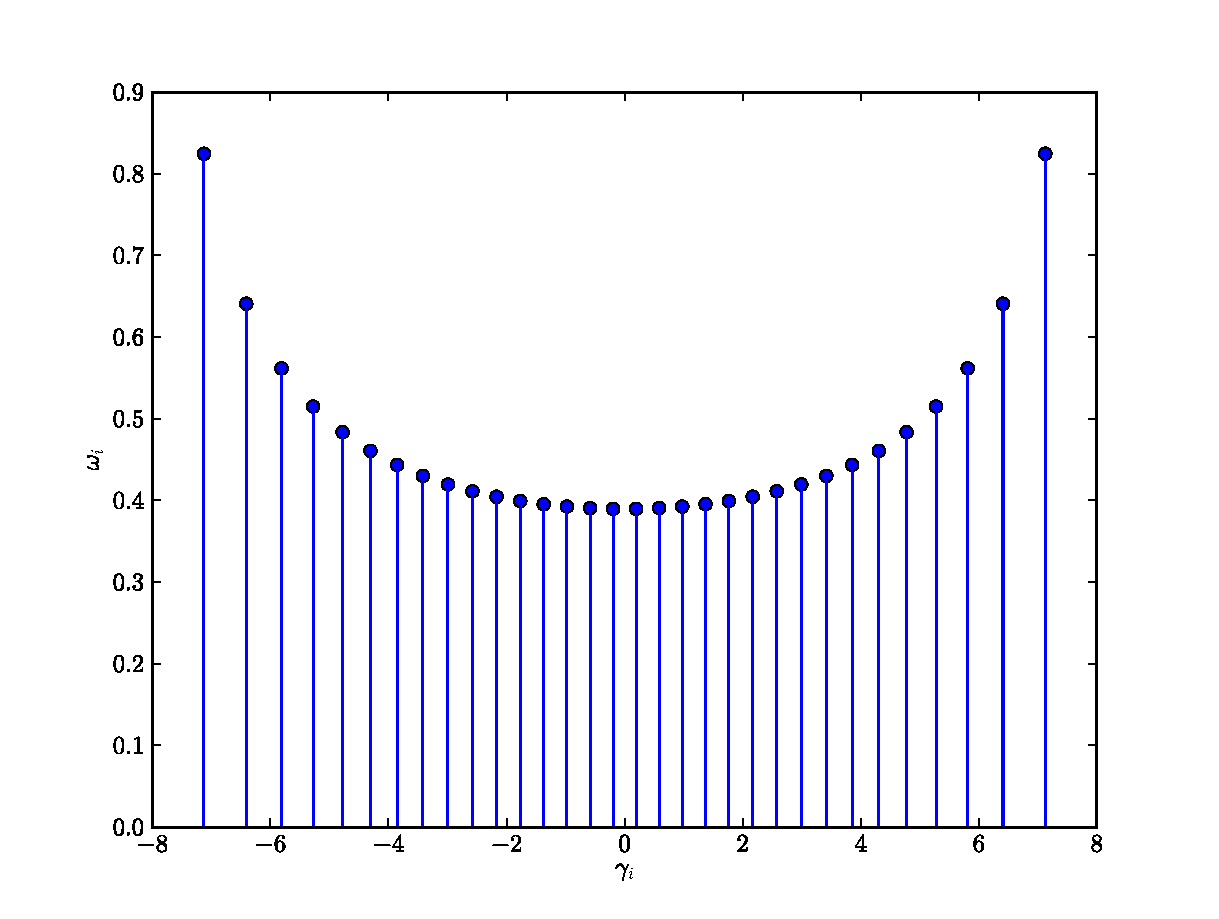
\includegraphics[width=0.8\linewidth]{./figures/quadrature_nodes.pdf}
  \caption{Example of transformed Qauss-Hermite quadrature weights.}
  \label{fig:quadrature_nodes}
\end{figure}

However, the nodes still deserve our attention. As we see in the figure \ref{fig:quadrature_nodes}
the nodes are centred around $0$. This is correct for integrating with a weighting function
$w\ofs{x} = e^{-x^2}$. But the Gaussian exponential present in our wavepacket's basis functions
given by \eqref{eq:hagedorn_groundstate_1d} is shifted away from $0$ by an amount $q$.
Hence we have to shift and spread the quadrature nodes as well:

\begin{equation}
  \gamma_i^\prime \assign q + \varepsilon |Q| \gamma_i \,.
\end{equation}

The figure \ref{fig:quadrature_nodes_single} shows an example of a quadrature for
an arbitrary homogeneous wavepacket $\Ket{\Psi}$ with parameters $\Pi = \left(i,3,0,0.4,2\right)$
and coefficients $c_0 = 0.25$, $c_1 = 0.3$ and $c_4 = 0.1$.

Anytime we need quadrature nodes and weights,
we'll use the pairs $\left(\gamma_i^\prime, \omega_i^\prime\right)$. After this
lengthy section about integration we return to the propagation algorithm.

\begin{figure}
  \centering
  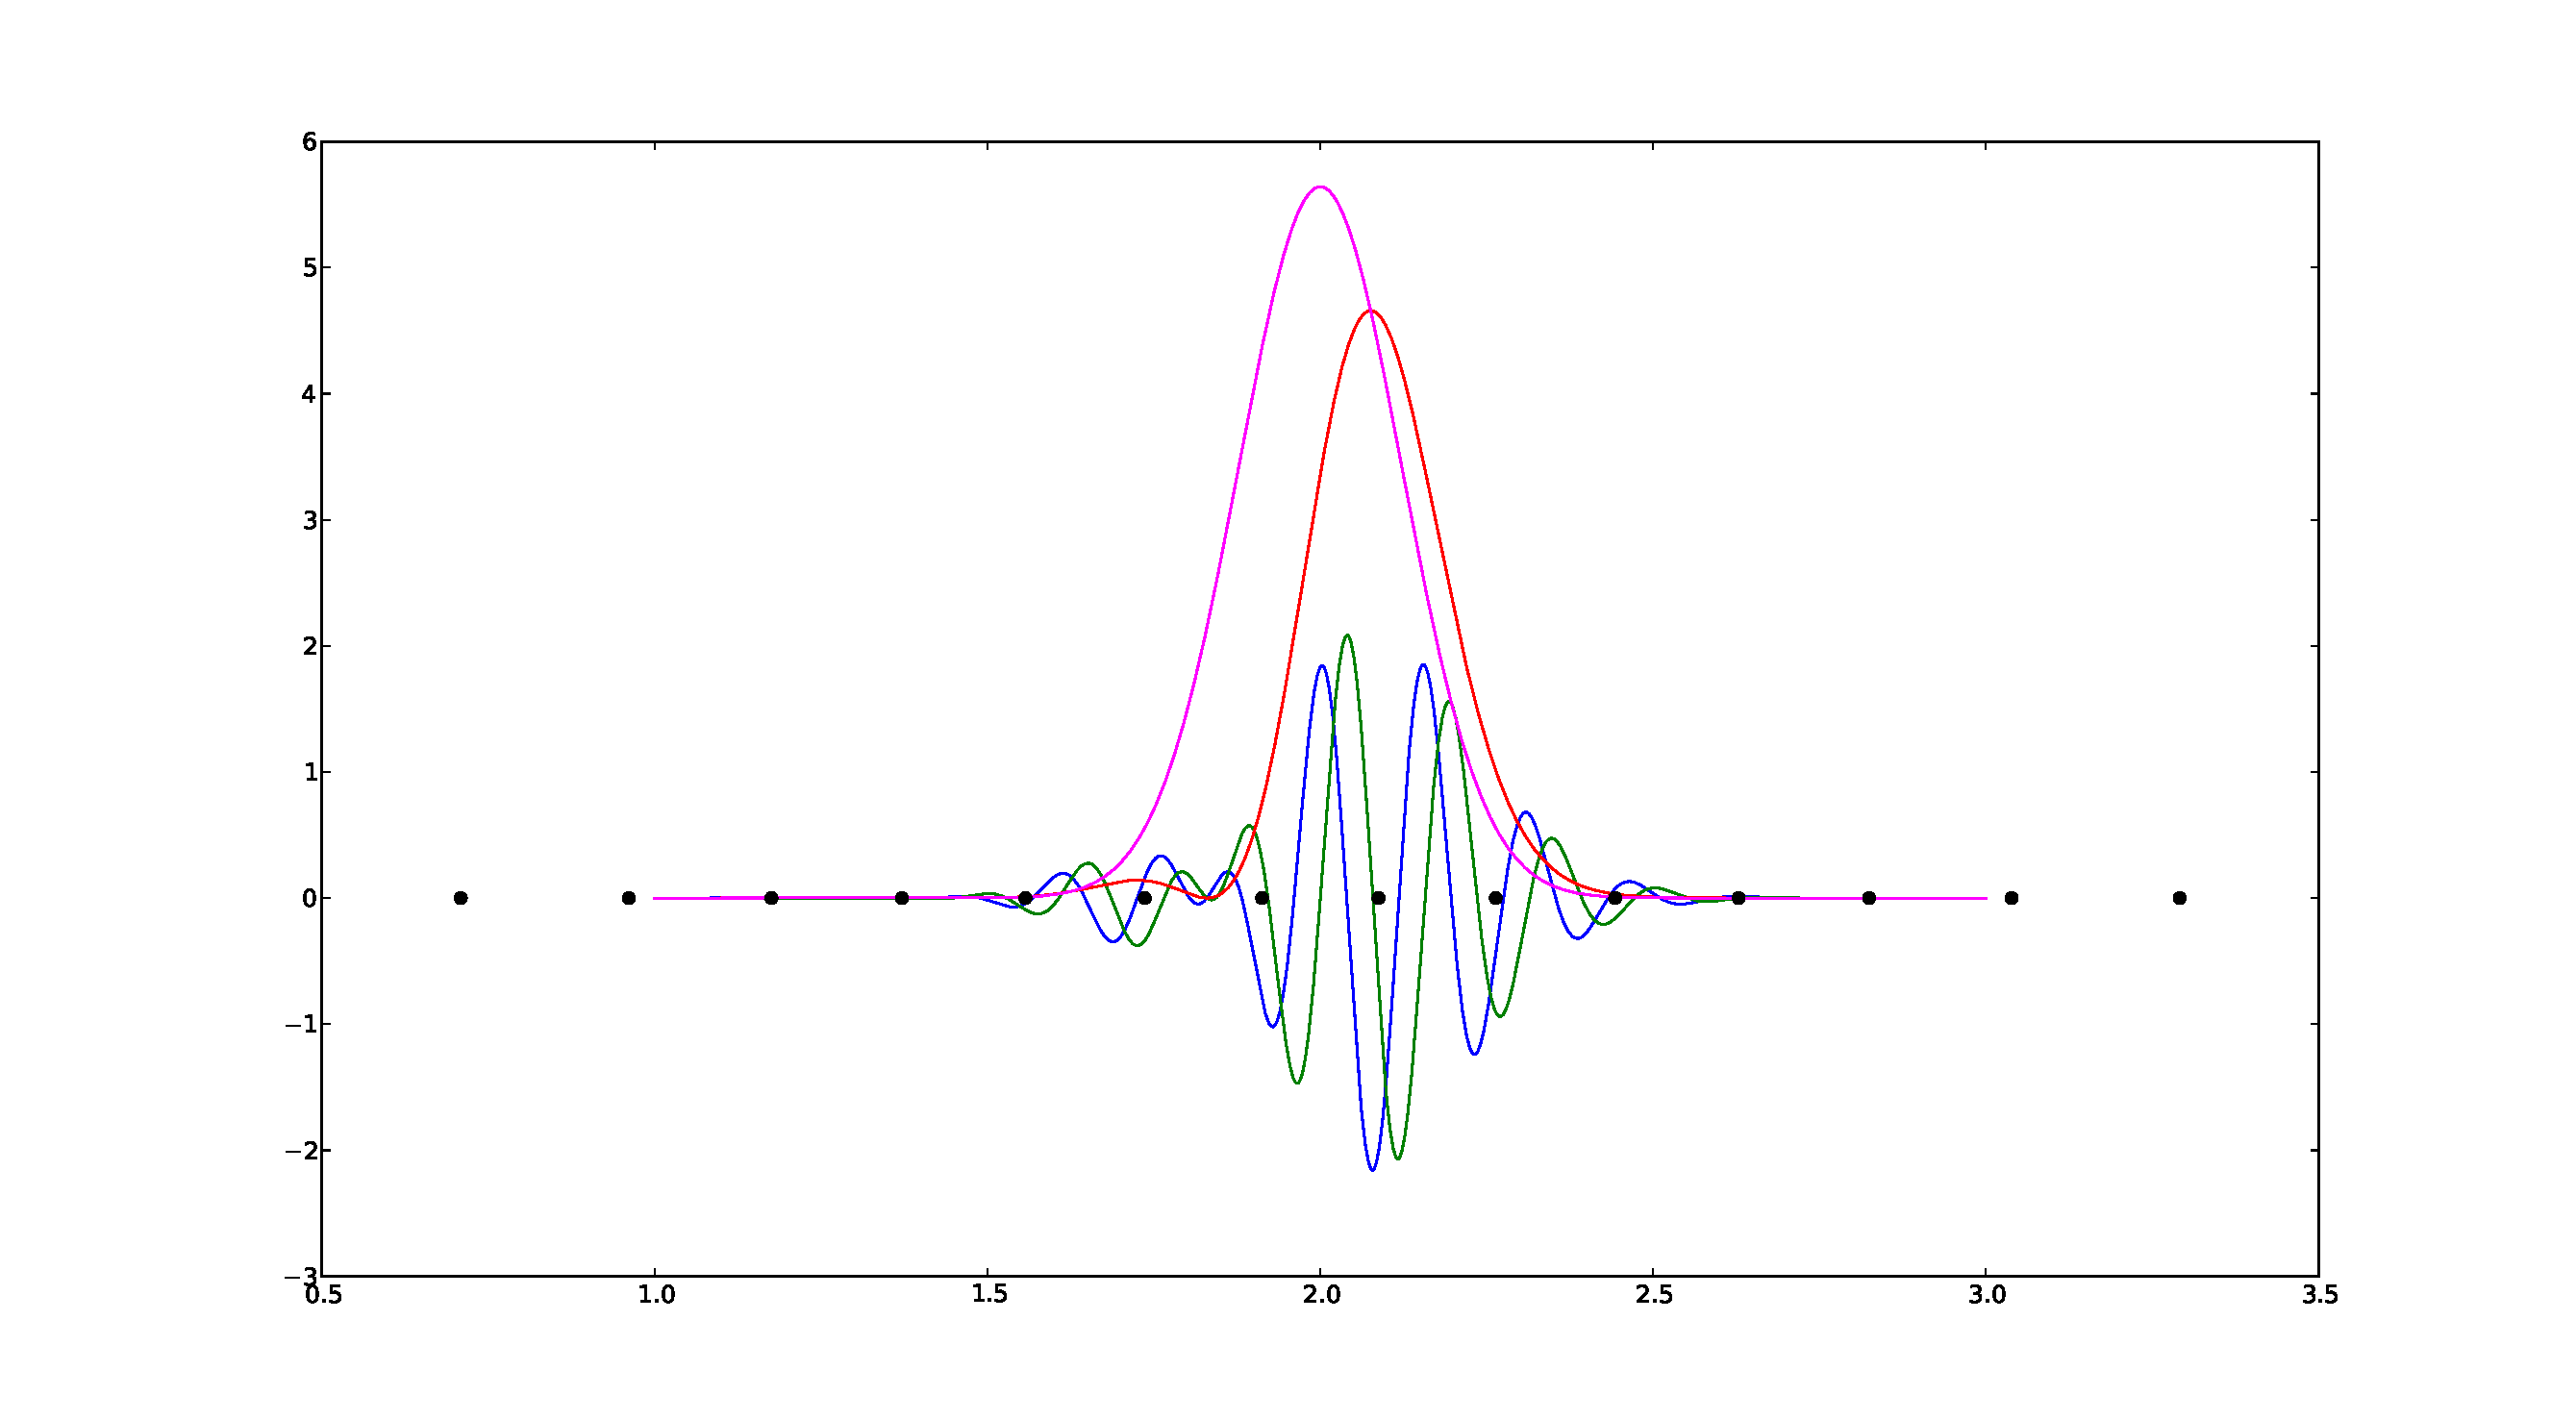
\includegraphics[width=\linewidth]{./figures/quadrature_nodes_single.pdf}
  \caption{Example of a quadrature for a given wavepacket $\Psi$ with. Plotted is
  the real (blue) and imaginary (green) part as well as the absolute value (red) of
  the wavepacket. The black dots are the quadrature nodes. The magenta curve shows
  the Gaussian we get for a wavepacket with the same Hagedorn parameters $\Pi$ but
  $c_0 = 1$ and $c_{k>0} = 0$.}
  \label{fig:quadrature_nodes_single}
\end{figure}

\section{The original time propagation algorithm}
\label{sec:scalar_time_propagation}

Let us now review the time propagation algorithm briefly. The algorithm as defined
in section 3.3 of reference \cite{FGL_semiclassical_dynamics} is constructed for
the propagation of semiclassical wavepackets as defined by \eqref{eq:hawp_def_single}
in an arbitrary number of space dimensions. It integrates the three steps
\eqref{eq:splitting_prop_kinetic}, \eqref{eq:splitting_prop_harmonic} and \eqref{eq:splitting_prop_remainder}
and combines them into a propagation algorithm suitable for general potentials.

Given the parameters $P^{\left(j\right)}$, $Q^{\left(j\right)}$, the phase $S^{\left(j\right)}$
and the position $q^{\left(j\right)}$ and momentum $p^{\left(j\right)}$ of the state $\Ket{\Phi}$
at time $t^{\left(j\right)} \assign j \tau$ then the algorithm \ref{al:tp_wave_packets_scalar}
will compute the same values one time step $\tau$ later. We omitted the mass matrix $M$ here
that is present in ref. \cite{FGL_semiclassical_dynamics}. The whole algorithm essentially
only propagates the Hagedorn parameters and the coefficients in time.

\begin{algorithm}
\caption{Time propagation of scalar wavepackets $\Ket{\Phi}$}
\label{al:tp_wave_packets_scalar}
\begin{algorithmic}
  \REQUIRE A semiclassical wavepacket $\Ket{\Phi\ofs{t}}$ with its Hagedorn parameters
  \STATE // Propagate with the kinetic operator
  \STATE $q^{\left(j+\frac{1}{2}\right)} \assign q^{\left(j\right)} + \frac{\tau}{2} p^{\left(j\right)}$
  \STATE $Q^{\left(j+\frac{1}{2}\right)} \assign Q^{\left(j\right)} + \frac{\tau}{2} P^{\left(j\right)}$
  \STATE $S^{\left(j+\frac{1}{2},-\right)} \assign S^{\left(j\right)} + \frac{\tau}{4} p^{\left(j\right)}\T p^{\left(j\right)}$
  \STATE // Propagate with the local quadratic potential
  \STATE $p^{\left(j+1\right)} \assign p^{\left(j\right)} - \tau \, \nabla V\ofs{q^{\left(j+1/2\right)}}$
  \STATE $P^{\left(j+1\right)} \assign P^{\left(j\right)} - \tau \, \nabla^2 V\ofs{q^{\left(j+1/2\right)}} Q^{\left(j+1/2\right)}$
  \STATE $S^{\left(j+1/2,+\right)} \assign S^{\left(j+1/2,-\right)} - \tau \, V\ofs{q^{\left(j+1/2\right)}}$
  \STATE // Propagate with the non-quadratic remainder
  \STATE // Assemble the matrix $F$
  \STATE $F_{k,l} \assign \Braket{\phi_k | W\ofs{x} | \phi_l} \quad \forall k,l \in 0,\ldots,K-1$
  \STATE // And propagate the coefficients
  \STATE $c^{\left(j+1\right)} \assign \exp\ofs{-\tau \frac{i}{\varepsilon^2} F^{\left(j+1/2\right)}} c^{\left(j\right)}$
  \STATE // Propagate with the kinetic operator again
  \STATE $q^{\left(j+1\right)} \assign q^{\left(j+1/2\right)} + \frac{\tau}{2} p^{\left(j+1\right)}$
  \STATE $Q^{\left(j+1\right)} \assign Q^{\left(j+1/2\right)} + \frac{\tau}{2} P^{\left(j+1\right)}$
  \STATE $S^{\left(j+1\right)} \assign S^{\left(j+1/2,+\right)} + \frac{\tau}{4} p^{\left(j+1\right)}\T p^{\left(j+1\right)}$
  \RETURN $\Ket{\Phi\ofs{t+\tau}}$
\end{algorithmic}
\end{algorithm}

\section{The propagation algorithm for vector valued wavepackets}

In this section we discuss what parts have to be altered in the algorithm \ref{al:tp_wave_packets_scalar}
such that we can propagate the vector valued wavepackets given by \eqref{eq:hawp_def_state_vector}.

What changes when we plug in the vector $\Ket{\Psi}$? First of all, the potential $V$
is now a matrix and we have to define carefully what we mean e.g. by $\nabla V$.
The vector of wavepackets defined by \eqref{eq:hawp_def_state_vector} has $N$
states. Thus we have $N$ vectors $c^0, \ldots, c^{N-1}$ each containing the coefficients
$c_k^{n}$ of the component $n$. On the other hand we have just a single set of
Hagedorn parameters $P$, $Q$, $S$, $p$ and $q$. From this first glance we can identify
the two core points. Who is responsible for propagating the parameters and how do
we have to modify the matrix $F$ to fully reflect the existence of multiple
coefficient vectors.

\subsection{Splitting of the potential matrix}

First we choose a so called \emph{leading component index} $\chi \in \{0, \ldots, N-1\}$. Then the energy level
$\lambda_\chi$ is the one responsible for propagating the Hagedorn parameters of
our wavepacket. Thus this energy level $\lambda\chi\ofs{x}$ takes over the role of the scalar
potential function $V\ofs{x}$ from section \ref{sec:scalar_time_propagation}.

We split the potential eigenvalue $\lambda\chi\ofs{x}$ into a local quadratic part $u_\chi$
and a non-quadratic remainder $w_\chi$. This is done via a simple Taylor series expansion
up to second order around a given point $q$.

\begin{equation} \label{eq:pot_taylor_split_general}
\begin{split}
  u_\chi\ofs{x} & = \lambda_\chi\ofs{q}
               + \nabla \lambda_\chi \left( q \right) \left( x-q \right)
               + \frac{1}{2} \left( x-q \right)\T \nabla^2 \lambda_\chi \left( q \right) \left( x-q \right) \\
  w_\chi\ofs{x} & = \lambda_\chi\ofs{x} - u_\chi\ofs{x} \,.
\end{split}
\end{equation}

For a potential in one space dimension that therefore depends only on one single
variable, say $x$, this reduces to

\begin{equation} \label{eq:pot_taylor_split_1d}
\begin{split}
  u_\chi\ofs{x} & = \lambda_\chi|_{x=q} + \frac{d}{dx}\lambda_\chi|_{x=q}\ofs{x-q} + \frac{1}{2} \frac{d^2}{dx^2}\lambda_\chi|_{x=q} \ofs{x-q}^2 \\
  w_\chi\ofs{x} & = \lambda_\chi\ofs{x} - u_\chi\ofs{x} \,.
\end{split}
\end{equation}

We can now write the potential matrix as a pure quadratic diagonal part $U$
plus a non-quadratic remainder matrix $W$:

\begin{equation} \label{eq:potiential_splitting_leading}
  V =
  \begin{pmatrix}
    u_\chi & {}     & 0 \\
    {}     & \ddots & {} \\
    0      & {}     & u_\chi \\
  \end{pmatrix}
  +
  \begin{pmatrix}
    v_{0,0} - u_\chi & \hdots & v_{0,N-1} \\
    \vdots           & \ddots & \vdots \\
    v_{N-1,0}        & \hdots & v_{N-1,N-1} - u_\chi \\
  \end{pmatrix} \,.
\end{equation}

The first part $U$ is not used explicitly in the propagation algorithm. We just
propagate one set of Hagedorn parameters and this can be done with $u_\chi$ solely. But
the non-quadratic part $W$ is used for altering and mixing the coefficients $c^i$ of
all components $\Phi_i$ of $\Ket{\Psi}$. This is the answer to the first of the questions posed above.

\subsection{Extending the handling of coefficients}
\label{sec:extending_the_handling_of_coefficients}

For finding an answer to the second question too, we elaborate on how to build the matrix $F$ this time.
To begin with we construct a new data structure for the coefficients. As said above, our $\Ket{\Psi}$
consists of $N$ components each of them having a vector $c^i$ with the $K$ coefficients
corresponding to $\Phi_i$. We can stack all these column vectors and build
a block vector $C$ with all coefficients of all components inside

\begin{equation} \label{eq:stack_coefficient_vectors_homog}
  C \assign
  \left(
  \begin{array}{c|c|c}
    c_0^0, \hdots, c_{K-1}^0 & \hdots & c_0^{N-1}, \hdots, c_{K-1}^{N-1}
  \end{array}
  \right)\T \,.
\end{equation}

This vector has $N K$ entries. A compatible matrix $\mathbf{F}$ of size $N K \times N K$
is now needed. The matrix is in block form too and we can even calculate all the $K \times K$ blocks
individually.

\begin{equation} \label{eq:blocked_F_homog}
  \mathbf{F} \assign
  \left(
  \begin{array}{c|c|c}
    F_{0,0}   & \hdots & F_{0,N-1} \\
    \hline
    \vdots    &        & \vdots \\
    \hline
    F_{N-1,0} & \hdots & F_{N-1,N-1} \\
  \end{array}
  \right) \,.
\end{equation}

Each of the $F_{i,j}$ is nothing else than the matrix $F$ known from \eqref{eq:the_matrix_f}.
But we have to be careful with the middle part of the braket. This time, our $W$ from \eqref{eq:potiential_splitting_leading}
is a matrix thus we can't simply build $\mathbf{F}$ from identical copies of $F$
even if the basis function $\phi_k$ are the same for all $F_{i,j}$. Instead we have to
distribute the individual entries $W_{i,j}$ of $W$ across the blocks of $\mathbf{F}$.
Thus each block $F_{i,j}$ of \eqref{eq:blocked_F_homog} is given by $\int_\mathbb{R} \widetilde{F}_{i,j}\ofs{x} dx$ where

\begin{equation}
  \widetilde{F}_{i,j}\ofs{x} \assign W_{i,j}\ofs{x}
  \begin{pmatrix}
     {}     & \vdots                             & {} \\
     \hdots & \conj{\phi_k\ofs{x}} \phi_l\ofs{x} & \hdots \\
     {}     & \vdots                             & {} \\
\end{pmatrix} \,.
\end{equation}

For all the individual blocks we could use algorithm \ref{al:build_matrix_block},
fed with the appropriate entry $W_{i,j}$ of the non-quadratic remainder matrix $W$,
to build the submatrices $F_{i,j}$. A basic explicit implementation of these formulae
is given in the algorithm \ref{al:build_block_matrix_homog} below.

\begin{algorithm}
\caption{Build the homogeneous block matrix $\mathbf{F} \assign \left(F_{r,c}\right)_{r,c}$}
\label{al:build_block_matrix_homog}
\begin{algorithmic}
  \REQUIRE A homogeneous wavepacket $\Psi$
  \REQUIRE $W$ a $N \times N$ matrix of scalar functions
  \STATE // Initialize $\mathbf{F}$ as the zero-matrix
  \STATE $\mathbf{F} \in \mathbb{R}^{NK \times NK}, \quad \mathbf{F} \assign \mathbf{0}$
  \STATE // Evaluate the basis functions for all quadrature nodes $\gamma$ with algorithm \ref{al:evaluate_basis_functions}
  \STATE given $\Pi$ as $\{P,Q,S,p,q\}$
  \STATE $B \assign \left(\beta_0, \ldots, \beta_{K-1}\right)$
  \STATE // Iterate over all row and column blocks of this matrix
  \FOR{$r = 0$ \TO $N-1$}
    \FOR{$c=0$ \TO $N-1$}
      \STATE // Evaluate the function $W_{r,c}$ for all quadrature nodes $\gamma$
      \STATE $\left(v_0, \ldots, v_{L-1}\right) \assign W_{r,c}\ofs{\left(\gamma_0, \ldots, \gamma_{L-1}\right)}$
      \STATE // Set up a zero matrix
      \STATE $F \in \mathbb{R}^{K \times K}, \quad F \assign \mathbf{0}$
      \STATE // Iterate over all pairs $\left(\gamma_l, \omega_l\right)$
      \FOR{$l=0$ \TO $L-1$}
        \STATE $F \assign F + v_{l} \varepsilon \cdot B\herm B \cdot \omega_l$
      \ENDFOR
      \STATE // Insert the block $F$ into the block matrix $\mathbf{F}$
      \STATE $\mathbf{F}_{r,c} \assign F$
    \ENDFOR
  \ENDFOR
  \RETURN $\mathbf{F}$
\end{algorithmic}
\end{algorithm}

\subsection{Pseudo code for the time propagation}

Now we are ready to write a new code which is able to propagate $\Ket{\Psi}$. This
algorithm is a generalization of the time propagation given in algorithm \ref{al:tp_wave_packets_scalar}.
The core concepts stay the same, but the details are a little bit more complex as
we saw in the last sections.

\begin{algorithm}
\caption{Time propagation of a homogeneous wavepacket $\Ket{\Psi}$}
\label{al:tp_wave_packets_homog}
\begin{algorithmic}
  \REQUIRE A semiclassical wavepacket $\Ket{\Psi\ofs{t}}$
  \REQUIRE The set $\Pi$ of Hagedorn parameters of $\Psi$
  \STATE // Propagate with the kinetic operator
  \STATE $q^{\left(j+\frac{1}{2}\right)} \assign q^{\left(j\right)} + \frac{\tau}{2} p^{\left(j\right)}$
  \STATE $Q^{\left(j+\frac{1}{2}\right)} \assign Q^{\left(j\right)} + \frac{\tau}{2} P^{\left(j\right)}$
  \STATE $S^{\left(j+\frac{1}{2},-\right)} \assign S^{\left(j\right)} + \frac{\tau}{4} p^{\left(j\right)}\T p^{\left(j\right)}$
  \STATE // Propagate with the local quadratic potential
  \STATE $p^{\left(j+1\right)} \assign p^{\left(j\right)} - \tau \, \nabla \lambda_\chi\ofs{q^{\left(j+1/2\right)}}$
  \STATE $P^{\left(j+1\right)} \assign P^{\left(j\right)} - \tau \, \nabla^2 \lambda_\chi\ofs{q^{\left(j+1/2\right)}} Q^{\left(j+1/2\right)}$
  \STATE $S^{\left(j+1/2,+\right)} \assign S^{\left(j+1/2,-\right)} - \tau \, \lambda_\chi\ofs{q^{\left(j+1/2\right)}}$
  \STATE // Propagate with the non-quadratic remainder
  \STATE // Stack the coefficient vectors $c^n$ of all components
  \STATE $C^{\left(j\right)} \assign \left(c^0, \hdots, c^{N-1}\right)\T$
  \STATE // Assemble the block matrix $\mathbf{F}$ using algorithm \ref{al:build_block_matrix_homog}
  \STATE $\mathbf{F}^{\left(j+1/2\right)} \assign \left(F_{r,c}\right)_{r,c} \quad \forall r,c \in 0,\ldots,N-1$
  \STATE // Propagate the coefficients
  \STATE $C^{\left(j+1\right)} \assign \exp\ofs{-\tau \frac{i}{\varepsilon^2} \mathbf{F}^{\left(j+1/2\right)}} C^{\left(j\right)}$
  \STATE // Split the coefficients
  \STATE $\left(c^0, \ldots, c^{N-1}\right) \assign C^{\left(j+1\right)}$
  \STATE // Propagate with the kinetic operator again
  \STATE $q^{\left(j+1\right)} \assign q^{\left(j+1/2\right)} + \frac{\tau}{2} p^{\left(j+1\right)}$
  \STATE $Q^{\left(j+1\right)} \assign Q^{\left(j+1/2\right)} + \frac{\tau}{2} P^{\left(j+1\right)}$
  \STATE $S^{\left(j+1\right)} \assign S^{\left(j+1/2,+\right)} + \frac{\tau}{4} p^{\left(j+1\right)}\T p^{\left(j+1\right)}$
  \RETURN $\Ket{\Psi\ofs{t+\tau}}$
\end{algorithmic}
\end{algorithm}

\section{Basis transformations}
\label{sec:basis_transformation_hagedorn}

For some calculations we should be able to transform the wavepacket from the canonical basis
to the eigenbasis of the given potential $V$ and vice versa. For example we set the initial
values in the potentials' eigenbasis but perform the simulation in the canonical basis. So we now
investigate how such a basis transformation works.

Given a wavepacket as usual in the form of \eqref{eq:hawp_def_state_vector}. Further assume the matrix
$M \in \mathbb{R}^{N \times N}$ to be the matrix that diagonalizes the potential
according to \eqref{eq:general_spectral_transformation}. The general form of \eqref{eq:general_transformation_matirx}
can be written with all the entries as

\begin{equation}
  M \assign \begin{pmatrix}
              m_{0,0} & \cdots & m_{0,N-1} \\
              \vdots  &        & \vdots  \\
              m_{N-1,0} & \cdots & m_{N-1,N-1}
            \end{pmatrix} \,.
\end{equation}

In the following we try to transform $\Ket{\Psi}$ to the eigenbasis. We start with
calculating $M \Ket{\Psi}$, the action of $M$ on $\Psi$.

\begin{equation}
\begin{split}
  \Ket{\Psi^{\prime}} & = M \Ket{\Psi} \\
               & = \begin{pmatrix}
                     m_{0,0} & \cdots & m_{0,N-1} \\
                     \vdots  &        & \vdots  \\
                     m_{N-1,0} & \cdots & m_{N-1,N-1}
                   \end{pmatrix}
                   \Ket{\begin{pmatrix} \Phi_0 \\ \vdots \\ \Phi_{N-1} \end{pmatrix}} \\
               & = \Ket{\begin{pmatrix} m_{0,0} \Phi_0 + & \cdots & + m_{0,N-1} \Phi_{N-1} \\ & \vdots & \\ m_{N-1,0} \Phi_0 + & \cdots & + m_{N-1,N-1} \Phi_{N-1} \end{pmatrix}} \,.
\end{split}
\end{equation}

For the next steps we just consider the $j$\textsuperscript{th} component of this last expression.

\begin{equation}
\begin{split}
  m_{j,0} \Phi_0 + \cdots + m_{j,N-1} \Phi_{N-1}
  & =
  m_{j,0} e^{\frac{iS}{\varepsilon^2}} \sum_{k_0} c_{k_0}^0 \phi_{k_0} + \cdots + m_{j,N-1} e^{\frac{iS}{\varepsilon^2}} \sum_{k_{N-1}} c_{k_{N-1}}^{N-1} \phi_{k_{N-1}} \\
  & =
  e^{\frac{iS}{\varepsilon^2}} \left( \sum_{k_0} m_{j,0} c_{k_0}^0 \phi_{k_0} + \cdots + \sum_{k_{N-1}} m_{j,N-1} c_{k_{N-1}}^{N-1} \phi_{k_{N-1}} \right) \\
  & =
  e^{\frac{iS}{\varepsilon^2}} \sum_{k} \left( m_{j,0} c_{k}^0 + \cdots + m_{j,N-1} c_{k}^{N-1} \right) \phi_{k} \\
  & =
  e^{\frac{iS}{\varepsilon^2}} \sum_{k} \underbrace{\sum_l^{N-1} m_{j,l} c_{k}^l}_{c_k^\prime} \phi_{k}
  \rassign e^{\frac{iS}{\varepsilon^2}} \Phi^{\prime}_j \,.
\end{split}
\end{equation}

From the last line we see that we can represent the components of the transformed
wavepacket $\Ket{\Psi^\prime}$ again in Hagedorn form with unchanged basis functions
$\phi_i\left(x\right)$. However, this is not enough to transform the wavepacket
to the potential's eigenbasis as we missed the point that all $m_{i,j}$ depend on $x$!
Hence we additionally need to project the above result to the subspace spanned by
the basis functions $\phi_i\left(x\right)$. This is done as usual with the inner
product.

Denote the coefficients of the $j$\textsuperscript{th} component of the final wavepacket
with $d_i^j$. Then we can write:

\begin{equation}
\begin{split}
  d_p^j & = \Braket{\phi_p | \Phi^{\prime}_j } \\
        & = \Braket{\phi_p\left(x\right) | \sum_k \sum_l^{N-1} m_{j,l}\left(x\right) c_k^l \phi_k\left(x\right)} \\
  d_p^j & = \sum_k \sum_l^{N-1} c_k^l \Braket{\phi_p\left(x\right) | m_{j,l}\left(x\right) \phi_k\left(x\right)} \,.
\end{split}
\end{equation}

The part in the braket is just another inner product and, from the definition, we
write it as an integral:

\begin{equation}
  \Braket{\phi_p\left(x\right) | m_{j,l}\left(x\right) \phi_k\left(x\right)} = \int_\mathbb{R} \conj{\phi_p\left(x\right)} m_{j,l}\left(x\right) \phi_k\left(x\right) dx \,.
\end{equation}

We will calculate this integral by means of quadrature again. A straight forward
implementation that calculates $d_p^j$ for all $p \in 0 \ldots K-1$ and $j \in 0 \ldots N-1$
could be given by the code snippet \eqref{al:naive_quadrature}. Here we assume a
basis size of $K$.

\begin{algorithm}
\caption{Simple version of the basis transformation integral for $\Ket{\Psi}$}
\label{al:naive_quadrature}
\begin{algorithmic}
  \FOR{$j=0$ \TO $N-1$}
    \FOR{$p=0$ \TO $K-1$}
      \STATE $d_p^j \assign 0$
      \FOR{$k=0$ \TO $K-1$}
        \FOR{$l=0$ \TO $N-1$}
          \STATE $d_p^j \assign d_p^j + c_k^l \int_\mathbb{R} \conj{\phi_p\left(x\right)} m_{j,l}\left(x\right) \phi_k\left(x\right) dx$
        \ENDFOR
      \ENDFOR
    \ENDFOR
  \ENDFOR
\end{algorithmic}
\end{algorithm}

It would be cumbersome and very inefficient to implement the calculation this way.
Thus let's try to reformulate the problem as a matrix multiplication such that we
can perform it efficiently. First, we can interchange the order of summation and
notice that $m$ depends on $j$ and $l$ but (of course) not on $p$ and $k$. This
allows us to calculate the vector of the coefficients $d^j$ for fixed $j$ as a sum
over matrix multiplications.

\begin{equation}
  \begin{pmatrix}
    \vdots \\
    d_p^j \\
    \vdots
  \end{pmatrix}
  = \sum_l^{N-1}
  \begin{pmatrix}
    {}     & \vdots & {} \\
    \hdots & \Braket{\varphi_p|m_{j,l} \varphi_k} & \hdots \\
    {}     & \vdots & {} \\
  \end{pmatrix}
  \begin{pmatrix}
    \vdots \\
    c_l \\
    \vdots
  \end{pmatrix}
  \quad j = 1 \ldots N-1 \,.
\end{equation}

We can do much better and assemble a big matrix to perform the calculations for
all the $j$ components of $\Ket{\Psi^e}$ simultaneously.

\begin{equation}
  \left(\begin{array}{c}
    d^0 \\
    \hline
    \vdots \\
    \hline
    d^{N-1}
  \end{array}\right)
  =
  \left(
  \begin{array}{c|c|c}
    \Braket{\varphi|m_{0,0}|\varphi} & \hdots & \Braket{\varphi|m_{0,N-1}|\varphi} \\
    \hline
    \vdots & {} & \vdots \\
    \hline
    \Braket{\varphi|m_{N-1,0}|\varphi} & \hdots & \Braket{\varphi|m_{N-1,N-1}|\varphi} \\
  \end{array}\right)
  \left(\begin{array}{c}
    c^0 \\
    \hline
    \vdots \\
    \hline
    c^{N-1}
  \end{array}\right)
\end{equation}

The block matrix, let's call it $\mathbf{F}$, is of size $N K \times N K$ with $N^2$ individual
blocks of size $K \times K$. The vectors $\varphi$ consist of all the $K$ basis
functions. Because the wavepacket is homogeneous all the $\varphi$ are equivalent
thus in fact we have only a single $\varphi$.

Finally we see that the transformation to the eigenbasis is nothing else than multiplication
with a big matrix where each matrix element is an integral which can easily be
carried out by quadrature. We already met matrices of this structure in section \ref{sec:extending_the_handling_of_coefficients}
hence we can use the algorithm \ref{al:build_block_matrix_homog} to construct
our matrix $\mathbf{F}$. We only need to call the algorithm with the argument $M$ instead of $W$.

\section{Norm calculation for wavepackets}

This section deals with the calculation of norms. Suppose we have got a wavepacket
as defined by \eqref{eq:hawp_def_single} and now we want to compute the norm
$\norm{\Phi}^2$ of this wavepacket. From the definition we derive:

\begin{equation}
\begin{split}
  \|\Phi\|^2 & = \Braket{\Phi|\Phi}
              = \Braket{e^{\frac{iS}{\varepsilon^2}} \sum_k c_k \phi_k | e^{\frac{iS}{\varepsilon^2}} \sum_l c_l \phi_l} \\
             & = \Braket{\sum_k c_k \phi_k | \sum_l c_l \phi_l} \\
             & = \sum_k \conj{c_k} \sum_l c_l  \underbrace{\Braket{\phi_k | \phi_l}}_{= \delta_{k,l}} \\
             & = \sum_{k,l} \conj{c_k} c_l \delta_{k,l} = \sum_k \conj{c_k} c_k \\
             & = \norm{c}^2 \,.
\end{split}
\end{equation}

Remember that $\Braket{\cdot|\cdot}$ is sesquilinear. Therefore the global phase
cancels out. Additionally we used orthogonality of the basis functions $\phi_i$.

\subsection{Norm calculation for vectorial wavepackets}

Now we do the same calculation but for homogeneous vector valued wavepackets of
the form defined by \eqref{eq:hawp_def_state_vector}. This case can easily be reduced
to the previous one. Again we start from the basic definition of the norm.

\begin{equation}
\begin{split}
  \| \Psi \|^2 & = \Braket{\Psi|\Psi}
                = \Braket{\begin{pmatrix} \Phi_0 \\ \vdots \\ \Phi_{N-1} \end{pmatrix} | \begin{pmatrix} \Phi_0 \\ \vdots \\ \Phi_{N-1} \end{pmatrix}} \\
               & = \sum_i^{N-1} \Braket{\Phi_i | \Phi_i} = \sum_i^{N-1} \| \Phi_i \|^2 \\
               & = \sum_i^{N-1} \norm{c^i}^2 \,.
\end{split}
\end{equation}

From the last line we see that the norm is nothing else than the sum of the squared
norms of each component. This makes the computation as well as the implementation
trivial.

\section{Potential and kinetic energies}

In this section we want to have a closer look at the different energies and the
calculations thereof.

\subsection{Potential energy}

The potential energy of a wavepacket $\Ket{\Psi}$ that feels the potential $V\of{x}$
is per definition given as $\Braket{\Psi | V | \Psi}$. In our case, $\Ket{\Psi}$
is a vector of $N$ components and the potential is a matrix valued function as
defined by \eqref{eq:general_potential_matrix} or alternatively a matrix of scalar
functions.

If we go back to the definition, the potential energy is expressed by

\begin{equation}
\begin{split}
  \Braket{\Psi | V | \Psi}
%     & = \Braket{ \begin{pmatrix} \Phi_0 \\ \vdots \\ \Phi_{N-1} \end{pmatrix}
%                | \begin{pmatrix} {} & {} & {} \\ {} & V\ofs{x} & {} \\ {} & {} & {} \end{pmatrix}
%                | \begin{pmatrix} \Phi_0 \\ \vdots \\ \Phi_{N-1} \end{pmatrix}
%                } \\
      & = \Braket{ \begin{pmatrix} \Phi_0 \\ \vdots \\ \Phi_{N-1} \end{pmatrix}
                 | \begin{pmatrix}
                     v_{0,0} \ofs{x}   & \hdots & v_{0,N} \ofs{x} \\
                     \vdots            & {}     & \vdots \\
                     v_{N-1,0} \ofs{x} & \hdots & v_{N-1,N-1} \ofs{x} \\
                   \end{pmatrix}
                 | \begin{pmatrix} \Phi_0 \\ \vdots \\ \Phi_{N-1} \end{pmatrix}
                 } \\
      & = \Braket{ \begin{pmatrix} \Phi_0 \\ \vdots \\ \Phi_{N-1} \end{pmatrix}
                 | \begin{pmatrix} \sum v_{0,i} \Phi_i \\ \vdots \\ \sum v_{N-1,i} \Phi_i \end{pmatrix}
                 }
\end{split}
\end{equation}

and with a little bit additional linear algebra we get the more handy result

\begin{equation} \label{eq:hagedorn_pot_energy}
  \Braket{\Psi | V | \Psi} = \sum_i^{N-1} \sum_j^{N-1} \Braket{ \Phi_i | v_{i,j} | \Phi_j }
\end{equation}

thus effectively splitting the integral into a sum of integrals with only single
components involved.

This simple case occurs when both components in the bra and the ket are identical,
i.e. $\Braket{ \Phi_i | v_{i,i} | \Phi_i }$. And the more difficult case is
$\Braket{ \Phi_i | v_{i,j} | \Phi_j }$ where the off diagonal terms of $V$ appear.
Their effect is obviously some kind of mixing the different components $\Phi_i$
and $\Phi_j$ and we will find the coefficient vectors of both, $c^i$ and $c^j$ in
the resulting formula.

Both integrals can be handled by the algorithm \ref{al:efficient_quadrature_phi}
where we have to supply the correct $v_{i,j}\ofs{x}$ for $f$.

Notice that formula \eqref{eq:hagedorn_pot_energy} is valid in the canonical basis.
And we are interested in the energies of the components $\Phi_i$ as they are
in the eigenbasis. To overcome this restriction we just transform to the
eigenbasis by the equation \eqref{eq:general_spectral_transformation}:

\begin{equation}
\begin{split}
    \Braket{\Psi | V | \Psi} & = \Braket{\Psi | M\ofs{x} \Lambda\ofs{x} M^{-1}\ofs{x} | \Psi} \\
                             & = \Braket{\Psi M | \Lambda\ofs{x} | M\T \Psi} \\
                             & = \Braket{\Psi^\prime | \Lambda\ofs{x} | \Psi^\prime} \,.
\end{split}
\end{equation}

Notice that $\Ket{\Psi^\prime}$ is not in the potential's eigenbasis yet because a
projection to the subspace spanned by all Hagedorn basis functions $\phi_k$ is
still missing. Thus we need the multiplication by $\mathbf{F}$ that also includes
the transformation by $M$:

\begin{equation}
  \begin{split}
    \Braket{\Psi | V | \Psi} & = \Braket{\mathbf{F}\Psi | \Lambda\ofs{x} | \mathbf{F} \Psi} \\
                             & = \Braket{\Psi^e | \Lambda\ofs{x} | \Psi^e} \,.
\end{split}
\end{equation}

This finally results in

\begin{equation} \label{eq:potential_energy_eigen_homog}
  E_{\text{pot}} = \sum_i^{N-1} \Braket{ \Phi_i^e | \lambda_i | \Phi_i^e }
\end{equation}

where we are left with just a single sum over the diagonal components. From this
transformation we see that the overall potential energy is constant independently
of the basis. But of course the potential energies of the components $\Phi_i$ are
not.

\subsection{Kinetic energy}

The kinetic part of the energy of a homogeneous semiclassical wavepacket is given by

\begin{equation} \label{eq:hagedorn_kinetic}
  E_{\text{kin}} = \Braket{\Psi | T | \Psi}
\end{equation}

where $T$ is the kinetic operator as given by definition \eqref{eq:basics_def_ops}.
Recalling that $\Ket{\Psi}$ contains several states $\Phi_i$, we have to extend
the above expression as follows

\begin{align} \label{eq:hagedorn_kinetic_multi}
  \Braket{\Psi | T | \Psi} & = \Braket{ \begin{pmatrix} \Phi_0 \\ \vdots \\ \Phi_{N-1} \end{pmatrix}
                                      | \begin{pmatrix} T & {} & 0 \\ {} & \ddots & {} \\ 0 & {} & T \end{pmatrix}
                                      | \begin{pmatrix} \Phi_0 \\ \vdots \\ \Phi_{N-1} \end{pmatrix}
                                      } \nonumber \\
                           & = \Braket{ \begin{pmatrix} \Phi_0 \\ \vdots \\ \Phi_{N-1} \end{pmatrix}
                                      | \begin{pmatrix} T \Phi_0 \\ \vdots \\ T \Phi_{N-1} \end{pmatrix}
                                      } \nonumber \\
                           & = \sum_{i=0}^{N-1} \Braket{\Phi_i | T | \Phi_i} \,.
\end{align}

From the fact that $T$ is diagonal it becomes clear that the calculation of the
kinetic energy can be achieved by component wise integration for each state.

To finish the calculation of kinetic energies we need to know the action of the
kinetic operator $T$ on a wavepacket $\Phi_i$. This is not as easy as for the
potential where $V\ofs{x}$ just acts by multiplication. In the following we use
linearity of the sum and the differential operator

\begin{equation}
\begin{split}
  T \Phi & = -\frac{1}{2}\varepsilon^4 \frac{\partial^2}{\partial x^2} \Phi\ofs{x} \\
         & = -\frac{1}{2}\varepsilon^4 \frac{\partial^2}{\partial x^2} e^{\frac{iS}{\varepsilon^2}} \sum_{k=0}^{K-1} c_k \phi_k \\
         & = -\frac{1}{2}\varepsilon^4 e^{\frac{iS}{\varepsilon^2}} \sum_{k=0}^{K-1} c_k  \frac{\partial^2}{\partial x^2} \phi_k\ofs{x} \,.
\end{split}
\end{equation}

With algorithm \ref{al:derivative_of_phi} we can calculate the action of $T^\prime \assign -i \varepsilon^2\frac{\partial}{\partial x}$
on $\Phi$. Here the operator $T^\prime$ is a square root of $T$ up to the prefactor
$\frac{1}{2}$. We can apply it to both the bra and the ket of \eqref{eq:hagedorn_kinetic_multi}
individually:

\begin{equation} \label{eq:kinetic_energy_eigen_homog}
\begin{split}
  E_{\text{kin}} & = \sum_i \Braket{\Phi_i | T | \Phi_i} \\
                 & = \sum_i \Braket{\Phi_i | T^\prime\herm \left(\frac{1}{2}\right) T^\prime | \Phi_i} \\
                 & = \sum_i \frac{1}{2} \Braket{ T^\prime \Phi_i | T^\prime \Phi_i} \\
                 & = \frac{1}{2} \sum_i \| T^\prime \Phi_i \|^2 \,.
\end{split}
\end{equation}

Finally we need to transform the whole calculation to the eigenbasis. This is not
difficult. The last step shows that we can calculate the kinetic energy as the norm
of the coefficients of a transformed wavepacket $T^\prime \Phi$ individually for
each component. This allows us to transfer the wavepacket $\Ket{\Psi}$ to the eigenbasis
before we apply $T^\prime$.

\begin{algorithm}
\caption{Calculate the action of $T^\prime$ on a wavepacket $\Phi$}
\label{al:derivative_of_phi}
\begin{algorithmic}
  \REQUIRE A wavepacket $\Phi$ with coefficients $c_k$
  \STATE // Initialize a zero vector of length $K+1$
  \STATE $d \assign \left(0, \ldots, 0\right)$
  \STATE // Base cases
  \STATE $d_0 \assign d_0 + p c_0$
  \STATE $d_1 \assign d_1 + \sqrt{\frac{\varepsilon^2}{2}} P c_0$
  \STATE // Inductive steps
  \FOR{$k \assign 1$ \TO $K$}
    \STATE $d_k \assign d_k + p c_k$
    \STATE $d_{k+1} \assign d_{k+1} + \sqrt{k+1} \sqrt{\frac{\varepsilon^2}{2}} P c_k$
    \STATE $d_{k-1} \assign d_{k-1} + \sqrt{k} \sqrt{\frac{\varepsilon^2}{2}} \conj{P} c_k$
  \ENDFOR
  \RETURN $c \assign \left(d_0, \ldots, d_{K-1}\right)$
\end{algorithmic}
\end{algorithm}
